\documentclass{standalone}
\usepackage{tikz}
\usetikzlibrary{patterns, positioning}
\usepackage[sfdefault]{ClearSans} %% option 'sfdefault' activates Clear Sans as the default text font
\usepackage[T1]{fontenc}

\begin{document}
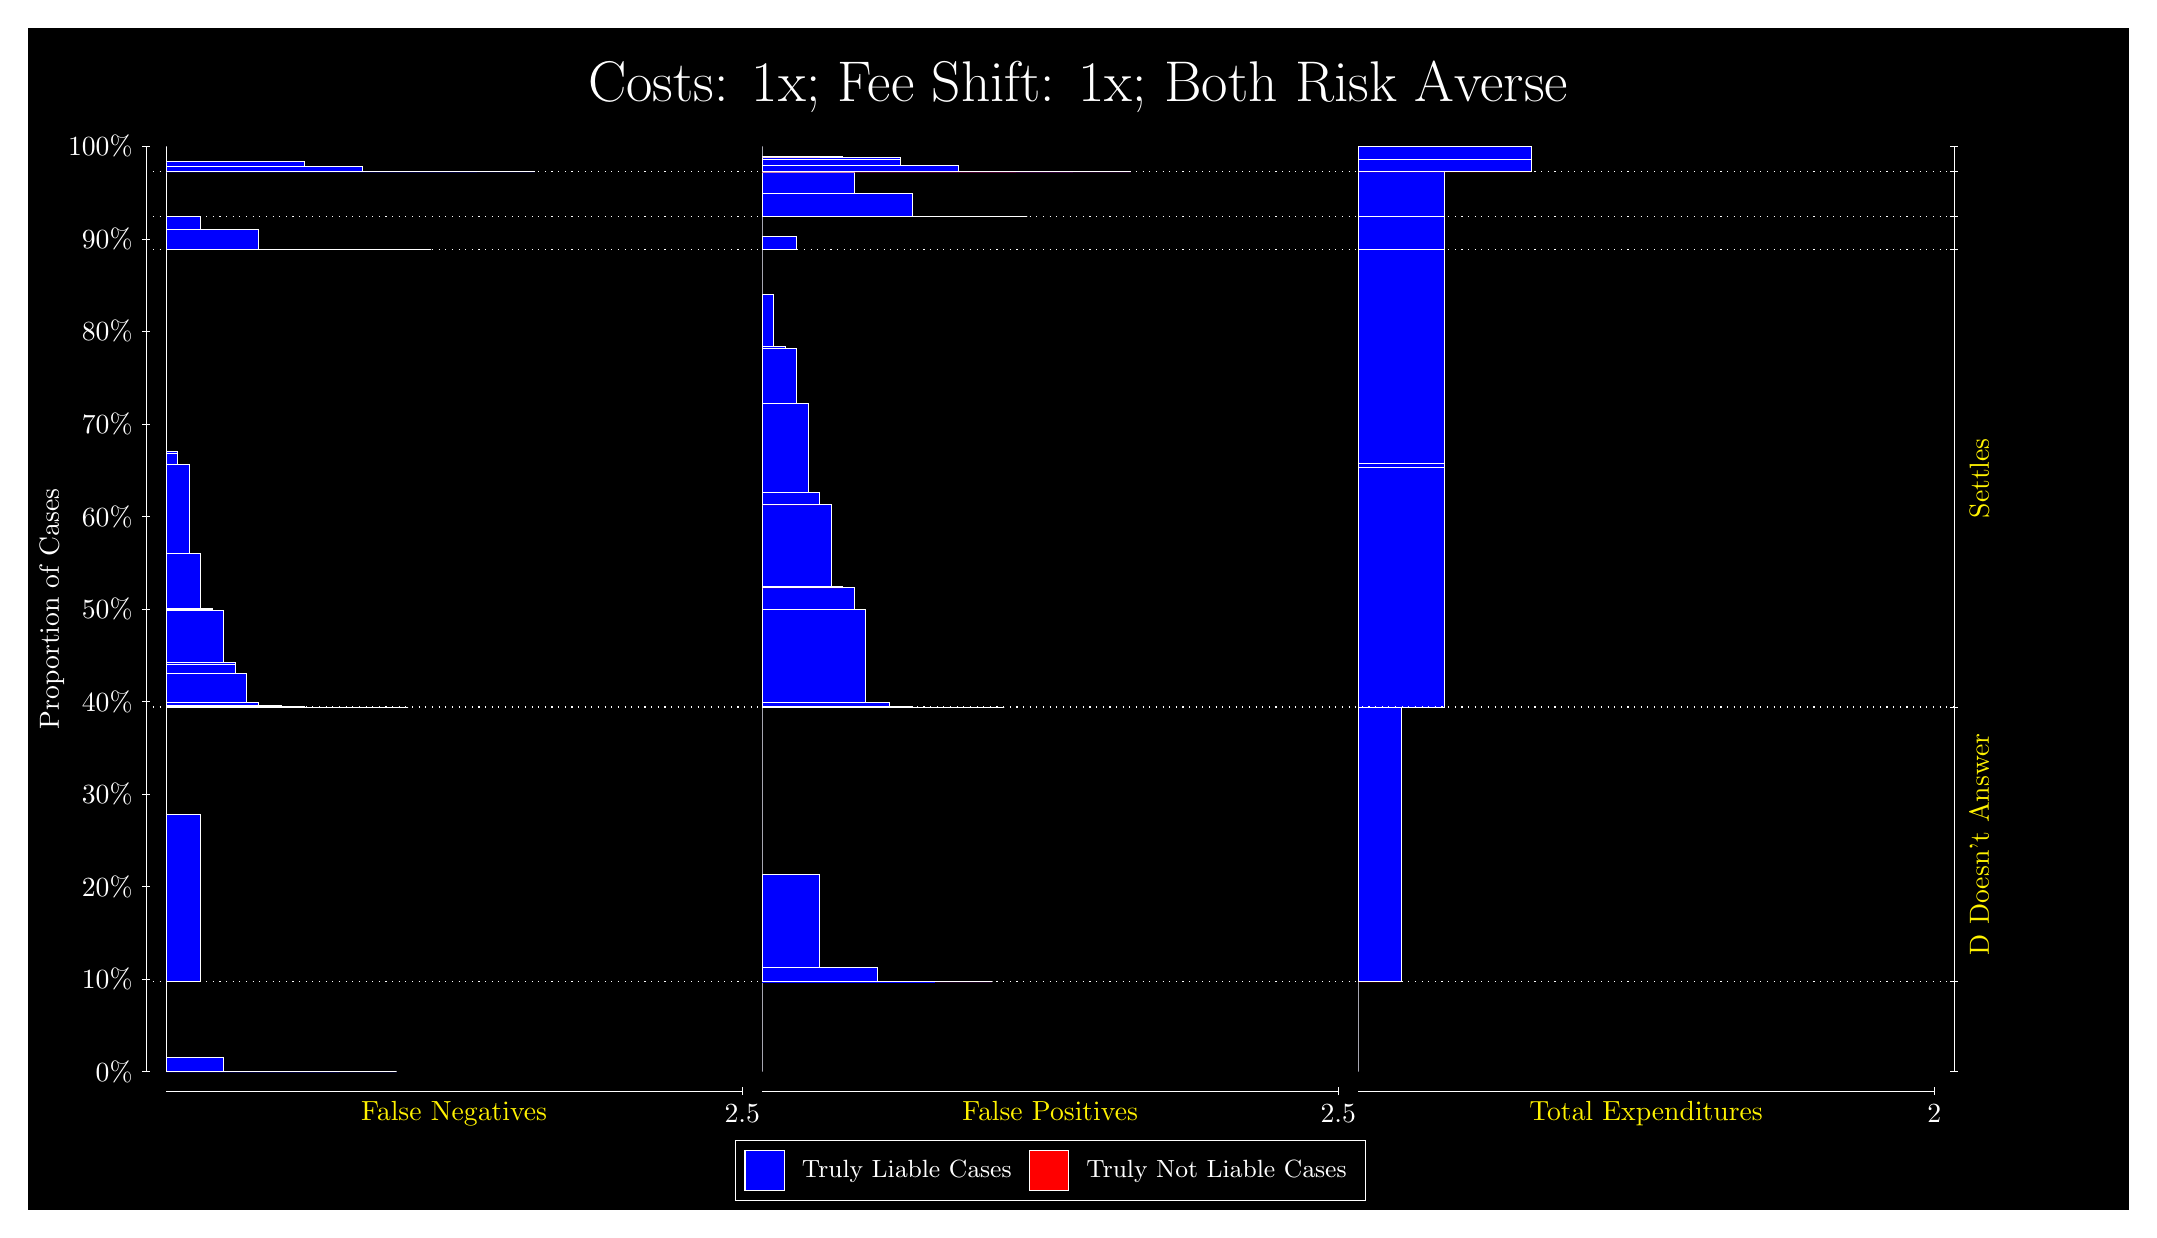
\begin{tikzpicture}
\draw[fill=black] (0,0) rectangle (26.667,15);
\draw[text=white] (0,13.5) rectangle (26.667,15) node[midway] {\huge Costs: 1x; Fee Shift: 1x; Both Risk Averse};
\draw[white, very thin] (1.5,1.75) -- (1.5,13.5);
\node[rotate=90, text=white, anchor=center] at (0.3, 7.625) {Proportion of Cases};
\draw[white, very thin] (1.45,1.75) -- (1.55,1.75);
\node[text=white, anchor=east] at (1.45, 1.75) {0\%};
\draw[white, very thin] (1.45,2.925) -- (1.55,2.925);
\node[text=white, anchor=east] at (1.45, 2.925) {10\%};
\draw[white, very thin] (1.45,4.1) -- (1.55,4.1);
\node[text=white, anchor=east] at (1.45, 4.1) {20\%};
\draw[white, very thin] (1.45,5.275) -- (1.55,5.275);
\node[text=white, anchor=east] at (1.45, 5.275) {30\%};
\draw[white, very thin] (1.45,6.45) -- (1.55,6.45);
\node[text=white, anchor=east] at (1.45, 6.45) {40\%};
\draw[white, very thin] (1.45,7.625) -- (1.55,7.625);
\node[text=white, anchor=east] at (1.45, 7.625) {50\%};
\draw[white, very thin] (1.45,8.8) -- (1.55,8.8);
\node[text=white, anchor=east] at (1.45, 8.8) {60\%};
\draw[white, very thin] (1.45,9.975) -- (1.55,9.975);
\node[text=white, anchor=east] at (1.45, 9.975) {70\%};
\draw[white, very thin] (1.45,11.15) -- (1.55,11.15);
\node[text=white, anchor=east] at (1.45, 11.15) {80\%};
\draw[white, very thin] (1.45,12.325) -- (1.55,12.325);
\node[text=white, anchor=east] at (1.45, 12.325) {90\%};
\draw[white, very thin] (1.45,13.5) -- (1.55,13.5);
\node[text=white, anchor=east] at (1.45, 13.5) {100\%};

\draw[white, very thin] (24.457,1.75) -- (24.457,13.5);
\draw[white, very thin] (24.407,1.75) -- (24.507,1.75);
\node[anchor=west] at (24.407, 1.75) {};
\draw[white, very thin] (24.407,2.8901) -- (24.507,2.8901);
\node[anchor=west] at (24.407, 2.8901) {};
\draw[white, very thin] (24.407,6.3791) -- (24.507,6.3791);
\node[anchor=west] at (24.407, 6.3791) {};
\draw[white, very thin] (24.407,12.19) -- (24.507,12.19);
\node[anchor=west] at (24.407, 12.19) {};
\draw[white, very thin] (24.407,12.611) -- (24.507,12.611);
\node[anchor=west] at (24.407, 12.611) {};
\draw[white, very thin] (24.407,13.178) -- (24.507,13.178);
\node[anchor=west] at (24.407, 13.178) {};
\draw[white, very thin] (24.407,13.5) -- (24.507,13.5);
\node[anchor=west] at (24.407, 13.5) {};

\draw[white, very thin, fill=blue] (1.75,1.75) rectangle (4.6775,1.75);
\draw[white, very thin, fill=blue] (1.75,1.75) rectangle (3.9457,1.75);
\draw[white, very thin, fill=blue] (1.75,1.75) rectangle (3.2138,1.7516);
\draw[white, very thin, fill=blue] (1.75,1.7516) rectangle (2.4819,1.9367);
\draw[white, very thin, fill=red] (1.75,1.9367) rectangle (1.75,1.9367);
\draw[white, very thin, fill=blue] (1.75,1.9367) rectangle (1.75,2.8901);
\draw[white, very thin, fill=blue] (1.75,2.8901) rectangle (2.1891,5.0166);
\draw[white, very thin, fill=red] (1.75,5.0166) rectangle (1.75,5.0166);
\draw[white, very thin, fill=blue] (1.75,5.0166) rectangle (1.75,6.3791);
\draw[white, very thin, fill=blue] (1.75,6.3791) rectangle (4.8239,6.3791);
\draw[white, very thin, fill=blue] (1.75,6.3791) rectangle (4.5312,6.3791);
\draw[white, very thin, fill=blue] (1.75,6.3791) rectangle (4.2384,6.3791);
\draw[white, very thin, fill=blue] (1.75,6.3791) rectangle (4.092,6.3791);
\draw[white, very thin, fill=blue] (1.75,6.3791) rectangle (3.9457,6.3791);
\draw[white, very thin, fill=blue] (1.75,6.3791) rectangle (3.7993,6.3791);
\draw[white, very thin, fill=blue] (1.75,6.3791) rectangle (3.6529,6.3791);
\draw[white, very thin, fill=blue] (1.75,6.3791) rectangle (3.5065,6.3887);
\draw[white, very thin, fill=blue] (1.75,6.3887) rectangle (3.3602,6.3897);
\draw[white, very thin, fill=blue] (1.75,6.3897) rectangle (3.2138,6.4053);
\draw[white, very thin, fill=blue] (1.75,6.4053) rectangle (3.0674,6.4054);
\draw[white, very thin, fill=blue] (1.75,6.4054) rectangle (3.0674,6.406);
\draw[white, very thin, fill=blue] (1.75,6.406) rectangle (2.921,6.4363);
\draw[white, very thin, fill=blue] (1.75,6.4363) rectangle (2.7746,6.8139);
\draw[white, very thin, fill=blue] (1.75,6.8139) rectangle (2.6283,6.9219);
\draw[white, very thin, fill=blue] (1.75,6.9219) rectangle (2.6283,6.9482);
\draw[white, very thin, fill=blue] (1.75,6.9482) rectangle (2.4819,7.6114);
\draw[white, very thin, fill=blue] (1.75,7.6114) rectangle (2.3355,7.6258);
\draw[white, very thin, fill=blue] (1.75,7.6258) rectangle (2.3355,7.6372);
\draw[white, very thin, fill=blue] (1.75,7.6372) rectangle (2.1891,8.3286);
\draw[white, very thin, fill=blue] (1.75,8.3286) rectangle (2.0428,9.4647);
\draw[white, very thin, fill=blue] (1.75,9.4647) rectangle (1.8964,9.6007);
\draw[white, very thin, fill=blue] (1.75,9.6007) rectangle (1.8964,9.6216);
\draw[white, very thin, fill=red] (1.75,9.6216) rectangle (1.75,9.6216);
\draw[white, very thin, fill=blue] (1.75,9.6216) rectangle (1.75,12.19);
\draw[white, very thin, fill=blue] (1.75,12.19) rectangle (5.1167,12.19);
\draw[white, very thin, fill=blue] (1.75,12.19) rectangle (4.3848,12.19);
\draw[white, very thin, fill=blue] (1.75,12.19) rectangle (3.6529,12.197);
\draw[white, very thin, fill=blue] (1.75,12.197) rectangle (2.921,12.442);
\draw[white, very thin, fill=blue] (1.75,12.442) rectangle (2.1891,12.611);
\draw[white, very thin, fill=red] (1.75,12.611) rectangle (1.75,12.611);
\draw[white, very thin, fill=blue] (1.75,12.611) rectangle (2.1891,12.614);
\draw[white, very thin, fill=red] (1.75,12.614) rectangle (1.75,12.614);
\draw[white, very thin, fill=blue] (1.75,12.614) rectangle (1.75,13.178);
\draw[white, very thin, fill=blue] (1.75,13.178) rectangle (6.4341,13.178);
\draw[white, very thin, fill=blue] (1.75,13.178) rectangle (5.7022,13.178);
\draw[white, very thin, fill=blue] (1.75,13.178) rectangle (4.9703,13.183);
\draw[white, very thin, fill=blue] (1.75,13.183) rectangle (4.2384,13.249);
\draw[white, very thin, fill=blue] (1.75,13.249) rectangle (3.9457,13.249);
\draw[white, very thin, fill=blue] (1.75,13.249) rectangle (3.5065,13.307);
\draw[white, very thin, fill=blue] (1.75,13.307) rectangle (3.2138,13.307);
\draw[white, very thin, fill=blue] (1.75,13.307) rectangle (2.7746,13.308);
\draw[white, very thin, fill=blue] (1.75,13.308) rectangle (2.4819,13.316);
\draw[white, very thin, fill=blue] (1.75,13.316) rectangle (2.0428,13.316);
\draw[white, very thin, fill=red] (1.75,13.316) rectangle (1.75,13.316);
\draw[white, very thin, fill=blue] (1.75,13.316) rectangle (1.75,13.5);
\draw[white, very thin, fill=red] (9.3189,1.75) rectangle (9.3189,1.75);
\draw[white, very thin, fill=blue] (9.3189,1.75) rectangle (9.3189,2.8901);
\draw[white, very thin, fill=red] (9.3189,2.8901) rectangle (12.246,2.8901);
\draw[white, very thin, fill=blue] (9.3189,2.8901) rectangle (12.246,2.8901);
\draw[white, very thin, fill=blue] (9.3189,2.8901) rectangle (11.515,2.8914);
\draw[white, very thin, fill=blue] (9.3189,2.8914) rectangle (10.783,3.0792);
\draw[white, very thin, fill=blue] (9.3189,3.0792) rectangle (10.051,4.2526);
\draw[white, very thin, fill=blue] (9.3189,4.2526) rectangle (9.3189,6.3791);
\draw[white, very thin, fill=red] (9.3189,6.3791) rectangle (12.393,6.3791);
\draw[white, very thin, fill=blue] (9.3189,6.3791) rectangle (12.393,6.3791);
\draw[white, very thin, fill=red] (9.3189,6.3791) rectangle (11.807,6.3791);
\draw[white, very thin, fill=blue] (9.3189,6.3791) rectangle (11.807,6.3791);
\draw[white, very thin, fill=blue] (9.3189,6.3791) rectangle (11.661,6.3791);
\draw[white, very thin, fill=red] (9.3189,6.3791) rectangle (11.515,6.3791);
\draw[white, very thin, fill=blue] (9.3189,6.3791) rectangle (11.515,6.3791);
\draw[white, very thin, fill=red] (9.3189,6.3791) rectangle (11.222,6.3791);
\draw[white, very thin, fill=blue] (9.3189,6.3791) rectangle (11.222,6.3887);
\draw[white, very thin, fill=blue] (9.3189,6.3887) rectangle (11.075,6.3888);
\draw[white, very thin, fill=red] (9.3189,6.3888) rectangle (10.929,6.3888);
\draw[white, very thin, fill=blue] (9.3189,6.3888) rectangle (10.929,6.4379);
\draw[white, very thin, fill=blue] (9.3189,6.4379) rectangle (10.783,6.4395);
\draw[white, very thin, fill=red] (9.3189,6.4395) rectangle (10.636,6.4395);
\draw[white, very thin, fill=blue] (9.3189,6.4395) rectangle (10.636,7.6199);
\draw[white, very thin, fill=blue] (9.3189,7.6199) rectangle (10.49,7.8952);
\draw[white, very thin, fill=red] (9.3189,7.8952) rectangle (10.344,7.8952);
\draw[white, very thin, fill=blue] (9.3189,7.8952) rectangle (10.344,7.9104);
\draw[white, very thin, fill=blue] (9.3189,7.9104) rectangle (10.197,8.9477);
\draw[white, very thin, fill=red] (9.3189,8.9477) rectangle (10.051,8.9477);
\draw[white, very thin, fill=blue] (9.3189,8.9477) rectangle (10.051,9.1045);
\draw[white, very thin, fill=blue] (9.3189,9.1045) rectangle (9.9044,10.241);
\draw[white, very thin, fill=blue] (9.3189,10.241) rectangle (9.758,10.932);
\draw[white, very thin, fill=blue] (9.3189,10.932) rectangle (9.6116,10.958);
\draw[white, very thin, fill=blue] (9.3189,10.958) rectangle (9.4652,11.621);
\draw[white, very thin, fill=blue] (9.3189,11.621) rectangle (9.3189,12.19);
\draw[white, very thin, fill=red] (9.3189,12.19) rectangle (9.758,12.19);
\draw[white, very thin, fill=blue] (9.3189,12.19) rectangle (9.758,12.358);
\draw[white, very thin, fill=blue] (9.3189,12.358) rectangle (9.3189,12.611);
\draw[white, very thin, fill=red] (9.3189,12.611) rectangle (12.686,12.611);
\draw[white, very thin, fill=blue] (9.3189,12.611) rectangle (12.686,12.611);
\draw[white, very thin, fill=blue] (9.3189,12.611) rectangle (11.954,12.614);
\draw[white, very thin, fill=blue] (9.3189,12.614) rectangle (11.222,12.9);
\draw[white, very thin, fill=blue] (9.3189,12.9) rectangle (10.49,13.175);
\draw[white, very thin, fill=blue] (9.3189,13.175) rectangle (9.758,13.178);
\draw[white, very thin, fill=red] (9.3189,13.178) rectangle (14.003,13.178);
\draw[white, very thin, fill=blue] (9.3189,13.178) rectangle (14.003,13.178);
\draw[white, very thin, fill=red] (9.3189,13.178) rectangle (13.271,13.178);
\draw[white, very thin, fill=blue] (9.3189,13.178) rectangle (13.271,13.178);
\draw[white, very thin, fill=red] (9.3189,13.178) rectangle (12.539,13.178);
\draw[white, very thin, fill=blue] (9.3189,13.178) rectangle (12.539,13.185);
\draw[white, very thin, fill=blue] (9.3189,13.185) rectangle (11.807,13.258);
\draw[white, very thin, fill=red] (9.3189,13.258) rectangle (11.807,13.258);
\draw[white, very thin, fill=blue] (9.3189,13.258) rectangle (11.807,13.258);
\draw[white, very thin, fill=blue] (9.3189,13.258) rectangle (11.075,13.334);
\draw[white, very thin, fill=blue] (9.3189,13.334) rectangle (11.075,13.362);
\draw[white, very thin, fill=red] (9.3189,13.362) rectangle (10.783,13.362);
\draw[white, very thin, fill=blue] (9.3189,13.362) rectangle (10.783,13.362);
\draw[white, very thin, fill=blue] (9.3189,13.362) rectangle (10.344,13.363);
\draw[white, very thin, fill=blue] (9.3189,13.363) rectangle (10.344,13.37);
\draw[white, very thin, fill=red] (9.3189,13.37) rectangle (10.051,13.37);
\draw[white, very thin, fill=blue] (9.3189,13.37) rectangle (10.051,13.371);
\draw[white, very thin, fill=blue] (9.3189,13.371) rectangle (9.6116,13.371);
\draw[white, very thin, fill=blue] (9.3189,13.371) rectangle (9.6116,13.371);
\draw[white, very thin, fill=red] (9.3189,13.371) rectangle (9.3189,13.371);
\draw[white, very thin, fill=blue] (9.3189,13.371) rectangle (9.3189,13.5);
\draw[white, very thin, fill=red] (16.888,1.75) rectangle (16.888,1.75);
\draw[white, very thin, fill=blue] (16.888,1.75) rectangle (16.888,2.8901);
\draw[white, very thin, fill=red] (16.888,2.8901) rectangle (17.437,2.8901);
\draw[white, very thin, fill=blue] (16.888,2.8901) rectangle (17.437,6.3791);
\draw[white, very thin, fill=red] (16.888,6.3791) rectangle (17.986,6.3791);
\draw[white, very thin, fill=blue] (16.888,6.3791) rectangle (17.986,9.4257);
\draw[white, very thin, fill=red] (16.888,9.4257) rectangle (17.986,9.4257);
\draw[white, very thin, fill=blue] (16.888,9.4257) rectangle (17.986,9.4735);
\draw[white, very thin, fill=red] (16.888,9.4735) rectangle (17.986,9.4735);
\draw[white, very thin, fill=blue] (16.888,9.4735) rectangle (17.986,12.19);
\draw[white, very thin, fill=red] (16.888,12.19) rectangle (17.986,12.19);
\draw[white, very thin, fill=blue] (16.888,12.19) rectangle (17.986,12.611);
\draw[white, very thin, fill=red] (16.888,12.611) rectangle (17.986,12.611);
\draw[white, very thin, fill=blue] (16.888,12.611) rectangle (17.986,13.178);
\draw[white, very thin, fill=red] (16.888,13.178) rectangle (19.083,13.178);
\draw[white, very thin, fill=blue] (16.888,13.178) rectangle (19.083,13.335);
\draw[white, very thin, fill=red] (16.888,13.335) rectangle (19.083,13.335);
\draw[white, very thin, fill=blue] (16.888,13.335) rectangle (19.083,13.5);
\draw[white, dotted] (1.5,2.8901) -- (24.457,2.8901);
\draw[white, dotted] (1.5,6.3791) -- (24.457,6.3791);
\draw[white, dotted] (1.5,12.19) -- (24.457,12.19);
\draw[white, dotted] (1.5,12.611) -- (24.457,12.611);
\draw[white, dotted] (1.5,13.178) -- (24.457,13.178);
\draw[white, very thin] (1.75,1.5) -- (9.0689,1.5);
\node[text=yellow, anchor=north] at (5.4094, 1.5) {False Negatives};
\draw[white, very thin] (9.0689,1.45) -- (9.0689,1.55);
\node[text=white, anchor=north] at (9.0689, 1.45) {2.5};

\draw[white, very thin] (9.3189,1.5) -- (16.638,1.5);
\node[text=yellow, anchor=north] at (12.978, 1.5) {False Positives};
\draw[white, very thin] (16.638,1.45) -- (16.638,1.55);
\node[text=white, anchor=north] at (16.638, 1.45) {2.5};

\draw[white, very thin] (16.888,1.5) -- (24.207,1.5);
\node[text=yellow, anchor=north] at (20.547, 1.5) {Total Expenditures};
\draw[white, very thin] (24.207,1.45) -- (24.207,1.55);
\node[text=white, anchor=north] at (24.207, 1.45) {2};


\node[text=yellow, centered, rotate=90] at (24.777, 4.6346) {D Doesn't Answer};
\node[text=yellow, centered, rotate=90] at (24.777, 9.2846) {Settles};




\draw (12.978300999999998,1.5) node[draw=none] (baseCoordinate) {};
\begin{scope}[align=center]
        \matrix[scale=0.5, draw=white, below=0.5cm of baseCoordinate, nodes={draw}, column sep=0.1cm]{
            \node[rectangle, draw, minimum width=0.5cm, minimum height=0.5cm, fill=blue] {}; &
            \node[draw=none, font=\small, text=white] (B) {Truly Liable Cases}; &
            \node[rectangle, draw, minimum width=0.5cm, minimum height=0.5cm, fill=red] {}; &
            \node[draw=none, font=\small, text=white] (B) {Truly Not Liable Cases}; \\
            };
\end{scope}

\end{tikzpicture}
\end{document}